\chapter{Peer Network Activity Management}
\label{chap:pam}

Il sistema \textbf{\ac{PAM}} è stato il primo progetto in cui sono state
adottate le \ac{PBC}, segnando una svolta importante nel modo di sviluppare le applicazioni in \textit{Peer Network}.
In precedenza, l’infrastruttura della piattaforma di integrazione \ac{ESI}, che accoglie al suo interno
le \ac{PBC}, seguiva un’architettura monolitica. Tuttavia, l’implementazione di \ac{PAM} ha offerto un contesto
ideale per sperimentare e testare questa nuova metodologia. Il successo ottenuto
durante questa fase sperimentale ha dimostrato l’efficacia delle \ac{PBC}, non solo nel migliorare la
flessibilità e modularità del sistema, ma anche nel semplificare i processi di sviluppo. Questo ha
portato alla decisione strategica di estendere l’approccio basato sulle \ac{PBC} a tutte le
\ac{SBS} progettate successivamente per i clienti, segnando un’evoluzione
significativa nell’architettura delle applicazioni aziendali.

In questo capitolo vengono approfonditi i concetti introdotti precedentemente, riguardanti
le applicazioni componibili, gli oggetti di business e le \ac{PBC}. Verrà esaminato come \textit{Peer Network} abbia
adottato e adattato questi principi nello sviluppo delle proprie \ac{SBS}, analizzandone la struttura
generale e il funzionamento. Successivamente, l’attenzione sarà focalizzata su \ac{PAM}, che rappresenta un
caso specifico di \ac{SBS}. Poiché \ac{PAM} e le \ac{SBS} condividono la stessa architettura strutturale basata sulle
\ac{PBC}, il sistema sarà utilizzato come esempio pratico per illustrare l’applicazione concreta di tali
concetti.

\section{Struttura di una Smart Business Solution}
\textit{Peer Network} utilizza Figura \ref{fig:sbs} e Figura \ref{fig:sbs-sap} per mostrare l'organizzazione delle
applicazioni componibili che sviluppa,
chiamate \ac{SBS} e progettate per diversi clienti e settori. Ciascuna
soluzione è composta da:
\begin{itemize}
    \item componenti backend, che integrano servizi e dati distribuiti su più piattaforme. Questa parte
    comprende inoltre la piattaforma di integrazione \ac{ESI}, responsabile della gestione delle \ac{PBC}
    necessarie;
    \item componenti frontend, sviluppati e successivamente distribuiti tramite la piattaforma Liferay\footnote{https://www.liferay.com/it/home}.
\end{itemize}

\begin{figure}
    \centering
    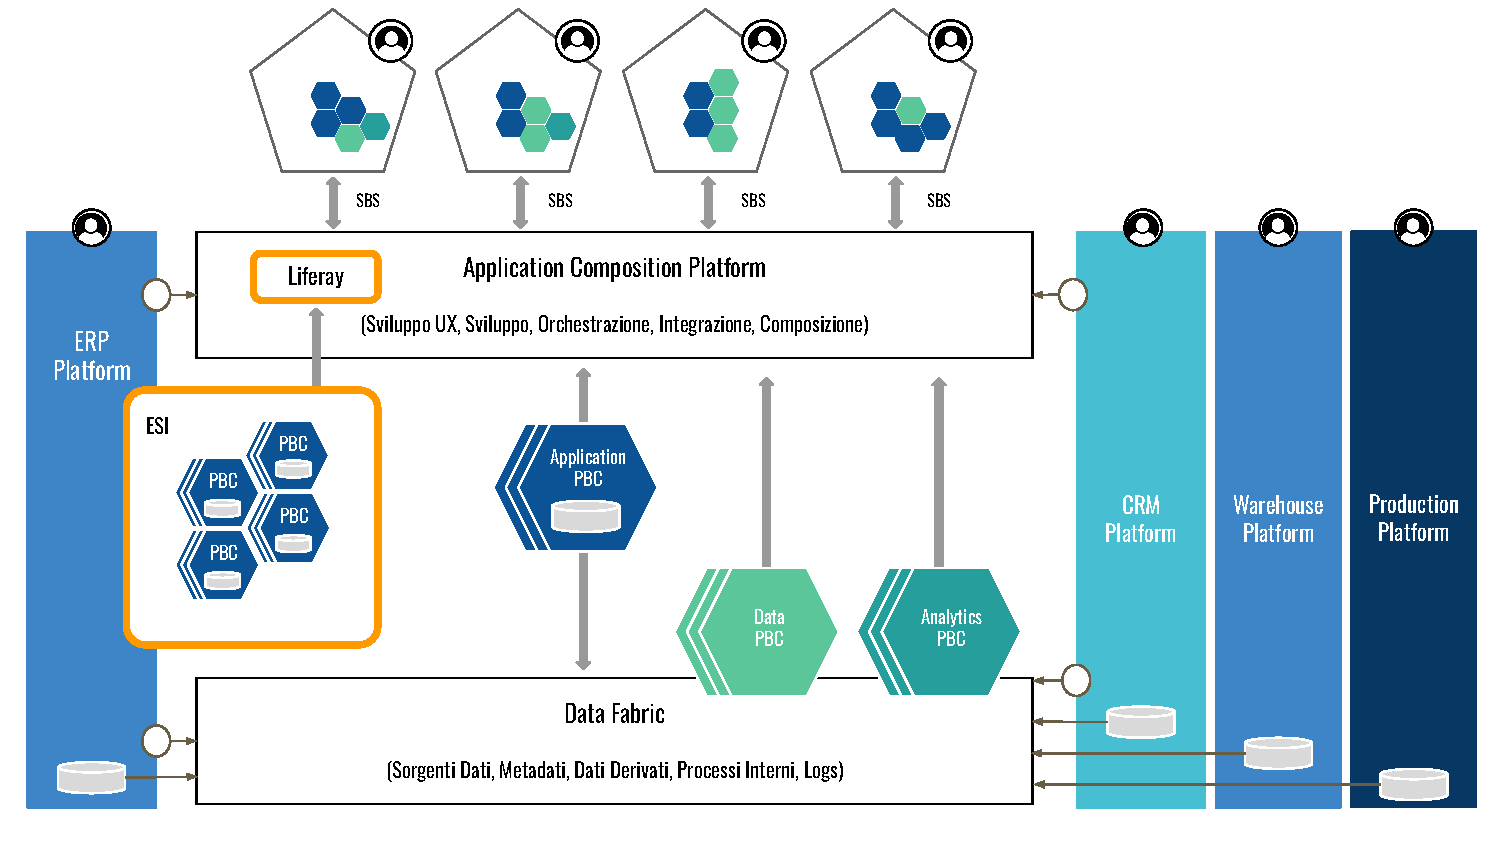
\includegraphics[width=\linewidth]{figures/struttura-sbs.pdf}
    \caption{Struttura di una \ac{SBS} e interazione tra i vari sistemi integrati}
    \label{fig:sbs}
\end{figure}

Dal punto di vista tecnico, ogni \ac{SBS} è composta da:
\begin{itemize}
    \item una parte di \textbf{backend}, che gestisce le logiche applicative ed è suddivisa in:
        \begin{itemize}
            \item \textbf{livello Data Fabric}, include sistemi informativi aziendali o database con cui la
            \ac{SBS} interagisce: ad esempio, può trattarsi di un \ac{ERP} (es. SAP), di un sistema \ac{CRM}
            (es. Salesforce) o di un database relazionale (es. MySQL). Poiché la maggior parte
            dei clienti utilizza sistemi SAP, le soluzioni si distinguono principalmente in SAP e non-SAP. In Figura
            \ref{fig:sbs-sap}, questo livello è rappresentato nella versione SAP;
            \item \textbf{livello \ac{PBC} Repository}, piattaforma \textbf{\ac{ESI}}: composto da \ac{PBC}, che forniscono accesso
            ai relativi dati e logiche applicative presenti nel livello Data Fabric. Le \ac{PBC}, pubblicate
            dalla piattaforma \ac{ESI}, fungono da intermediari tra le applicazioni e i sistemi informativi aziendali.
            A differenza di quanto formalizzato da Gartner, che individuava tre
            elementi base di una \ac{PBC}, dato, logiche e UI (opzionale), le \ac{PBC} di \textit{Peer Network} non contengono
            le rispettive interfacce utente, garantendo indipendenza tecnologica dal frontend. Sono state
            considerate due tipologie di \ac{PBC}:
            \begin{itemize}
                \item core: coprono funzionalità comuni a qualsiasi applicazione e cliente, quindi
                sono presenti in ogni \ac{SBS}. Nella Figura \ref{fig:sbs-sap} sono rappresentate dai cubi blu
                del livello PBC Repository;
                \item custom: realizzate per esigenze specifiche e applicazioni dedicate. Nella Figura \ref{fig:sbs-sap} sono rappresentate dai cubi
                arancioni del livello PBC Repository.
            \end{itemize}
            Le \ac{PBC} sono implementate come microservizi scritti in Kotlin\footnote{https://kotlinlang.org} e distribuite come container
            Docker\footnote{https://www.docker.com}, ciascuno contenente un gruppo coerente di \ac{PBC}. Ad esempio, G02 MATERIALS è il gruppo con
            funzionalità relative ai materiali, come il tipo di materiale PBC 0208 MATTYPE, la lista dei
            prezzi dei materiali PBC 0217 MATPRICELIST e l’unità di misura dei materiali PBC 0222 UNITOFMEASURE.
            In uno scenario on-premise (installazione presso il data-center del cliente), i
            microservizi sono orchestrati tramite Docker Compose. In uno scenario on-cloud, i
            microservizi vengono gestiti tramite Kubernetes\footnote{https://kubernetes.io}.
        \end{itemize}
    \item una parte di \textbf{frontend}, \textbf{Composable layer}, dedicata all’esperienza utente, il quale interagisce con
    la soluzione attraverso un'applicazione web.
    Anche il frontend viene realizzato come un insieme di moduli componibili (chiamati portlet)
    scritti in JavaScript utilizzando il framework Vue.js. Le portlet vengono assemblate in pagine web
    pubblicate tramite Liferay, seguendo un approccio componibile. Anche il frontend è gestito come
    microservizi, installati e orchestrati con modalità analoghe al livello \ac{PBC} Repository, sia in
    ambienti on-premise che cloud.
\end{itemize}

\begin{figure}
    \centering
    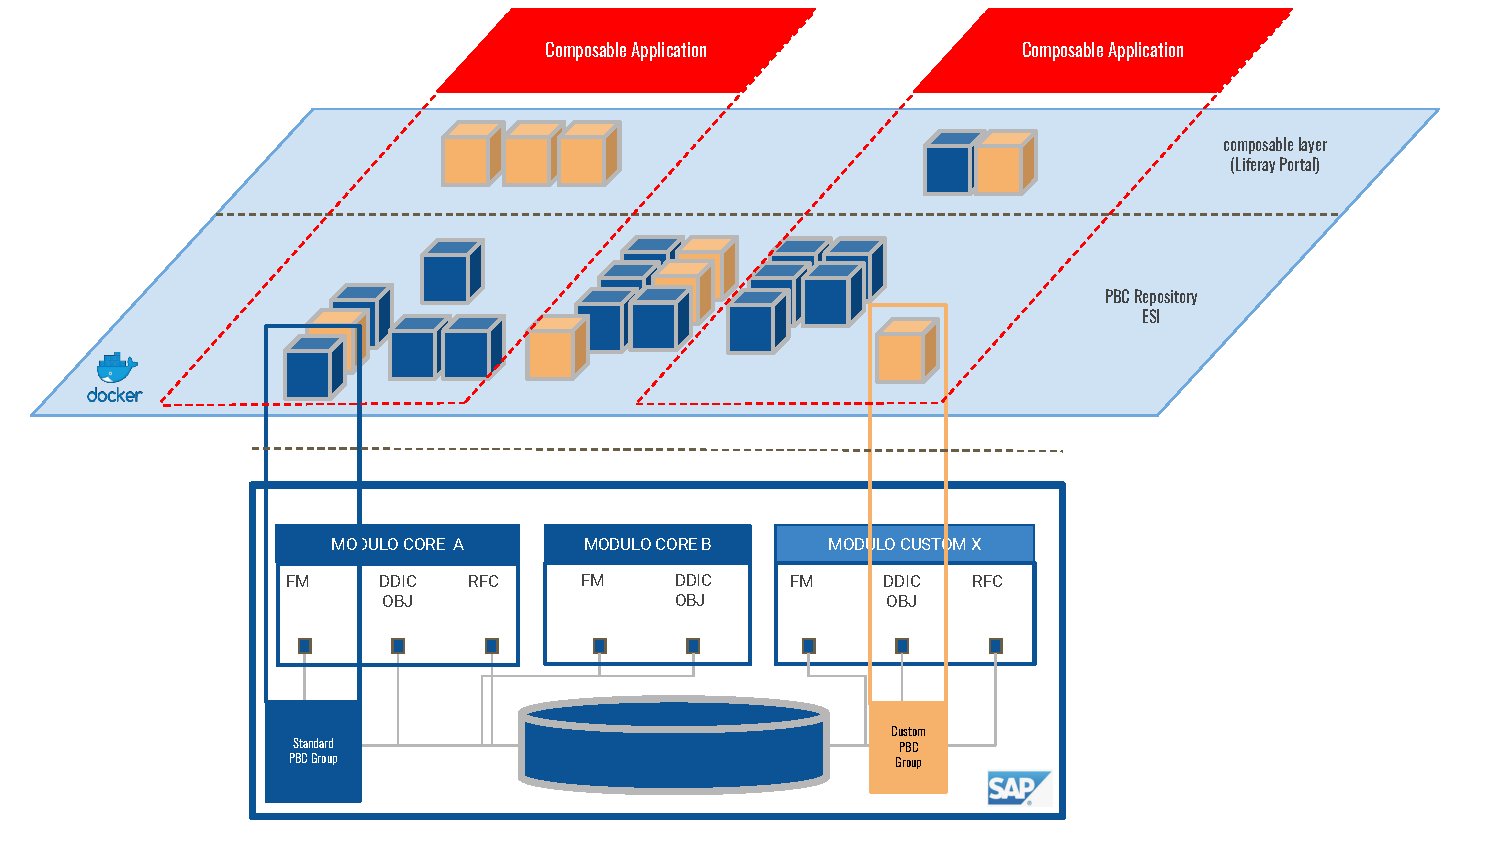
\includegraphics[width=\linewidth]{figures/architetturaSBS_SAP.pdf}
    \caption{Struttura di una \ac{SBS} che interagisce con un \ac{ERP} di SAP}
    \label{fig:sbs-sap}
\end{figure}

Entrando più nello specifico del livello \ac{PBC} Repository, la piattaforma \ac{ESI} gestisce le \ac{PBC}
attraverso due diversi livelli:
\begin{itemize}
    \item \textbf{livello API REST}: ospita i servizi di alto livello, cioè quelli riportati nella descrizione
    della \ac{PBC}. Questo strato è indipendente dallo scenario di implementazione ed è legato alla
    definizione dell’oggetto, così come la struttura dati;
    \item \textbf{livello sub-service}: ospita i servizi che interagiscono direttamente con lo strato dati
    della \ac{PBC}. I servizi implementati in questo livello differiscono a seconda del sistema informativo
    o database aziendale con il quale interagiscono:
    \begin{itemize}
        \item scenario SAP: i due layer API REST e sub-service sono gestiti da \ac{ESI} per SAP.
        In questo scenario il sub-service layer è costituito da BAPI, RFC e FM, oltre a servizi REST
        che interagiscono con la base dati dell'\ac{ERP} di SAP;
        \item scenario non-SAP: i due layer API REST e sub-service sono gestiti dalla versione
        di \ac{ESI} non-SAP. In questo scenario il sub-service layer è costituito da servizi che
        interagiscono con un database relazionale.
    \end{itemize}
\end{itemize}

    \subsection{Struttura di Peer Network Activity Management}
    Considerando l’architettura delle \ac{SBS} descritta in precedenza, \ac{PAM} è stata realizzata con:
    \begin{itemize}
        \item un modulo di backend che comprende:
        \begin{itemize}
            \item la base dati: come piattaforma per il database viene usato MySQL ed è installato presso il
            cloud provider OVH\footnote{https://www.ovhcloud.com} su una macchina proprietaria;
            \item le logiche che interagiscono con la base dati e i servizi relativi, viene usato
            \ac{ESI} non-SAP (installato presso il cloud provider OVH su una macchina proprietaria) come
            strumento di esposizione dei servizi e integrazione con le componenti di frontend.
        \end{itemize}
        \item un modulo di frontend che gestisce la UX/UI dell’applicazione, realizzato su
        Liferay Community Edition installato presso il cloud provider OVH su una macchina proprietaria.
    \end{itemize}
  
%figura?

\section{Attività svolte}

    \subsection{Sviluppo frontend}
    \subsection{Aggiornamento database}
    \subsection{Modifiche all’interfaccia grafica}
    \subsection{Implementazione di logica applicativa}